\documentclass{article}
\usepackage{parskip}
\usepackage{pdfpages}
\usepackage[margin=.6in]{geometry}

\begin{document}
We skipped a bunch of stuff cause its review of cs350. 


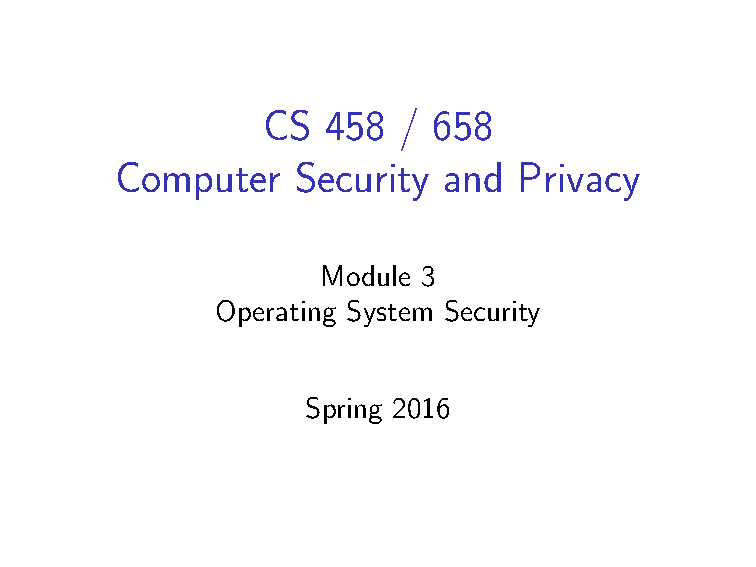
\includepdf[page=20]{Module3.pdf}
\textbf{Check every access} We want the OS to check everytime you try to access or it might notice that access had been revoked from you. Cause you're a dick.

\textbf{Enforcce least privilige} dont give people rights they dont need

\textbf{Verify acceptable use} limit the kinds of things people can do on objects

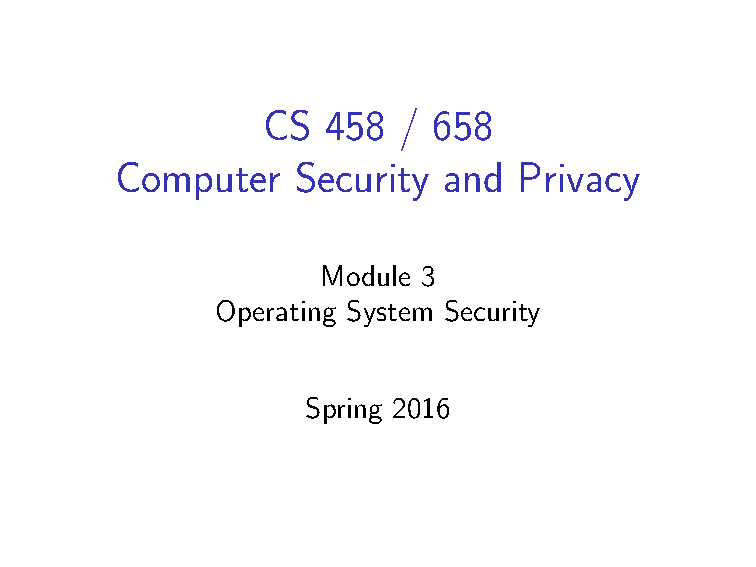
\includepdf[page=21-22]{Module3.pdf}
Most access control systems are visualized as a matrix (not implemented as one). Objects are things you want access to, Subjects are things trying to get access, and Rights are the things the subjects want to do to the object. 

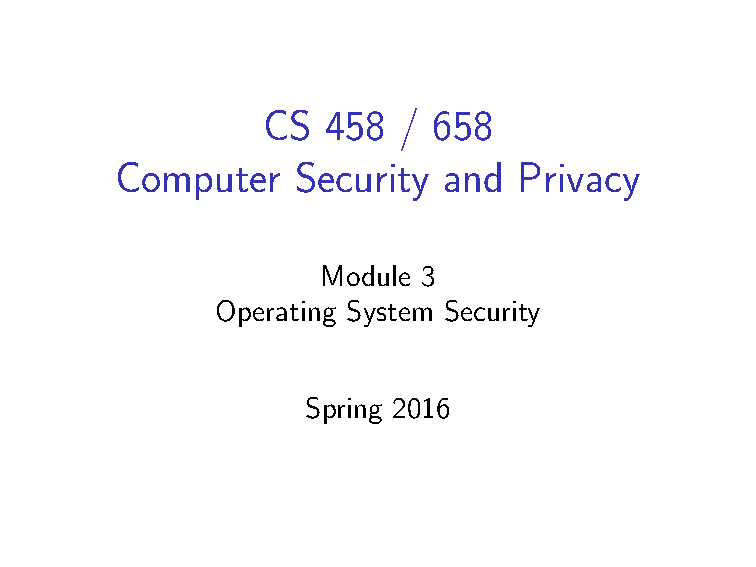
\includepdf[page=23]{Module3.pdf}
Iterating over the huge access control matrix is super inefficient because it tends to be a very sparse table. Instead we tend to work by columns or rows.

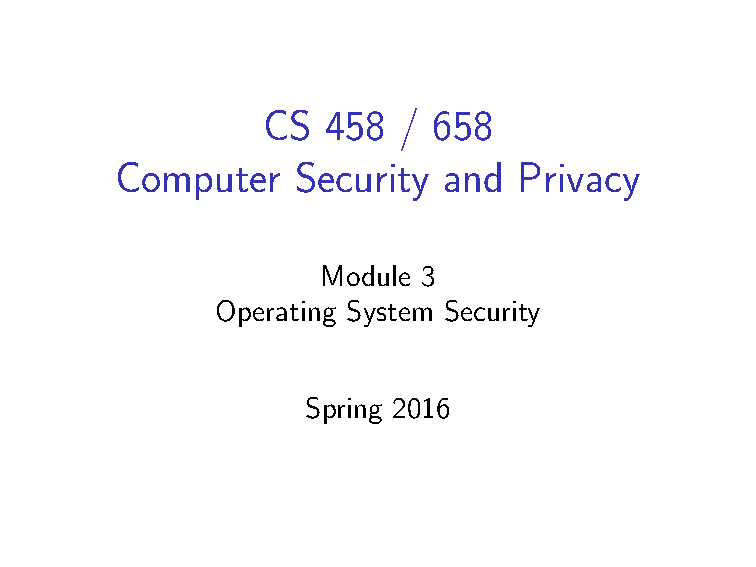
\includepdf[page=24]{Module3.pdf}
ACLs are what the UNIX system uses (chmod that shit). These are column wise interpretation of an access matrix.

\begin{itemize}
	\item o = owner
	\item g = group
	\item w = world
\end{itemize}

Looking at these ACLs:
\begin{itemize}
	\item we can easily find who is allowed to access an object: its very quick because this data is stored on the object
	\item we cannot easily find all objects a user can access: we'd have to go through all objects and check if the user can access it
	\item we can easily revoke access to a single object but stupid for all because you have to go through all of them
\end{itemize}

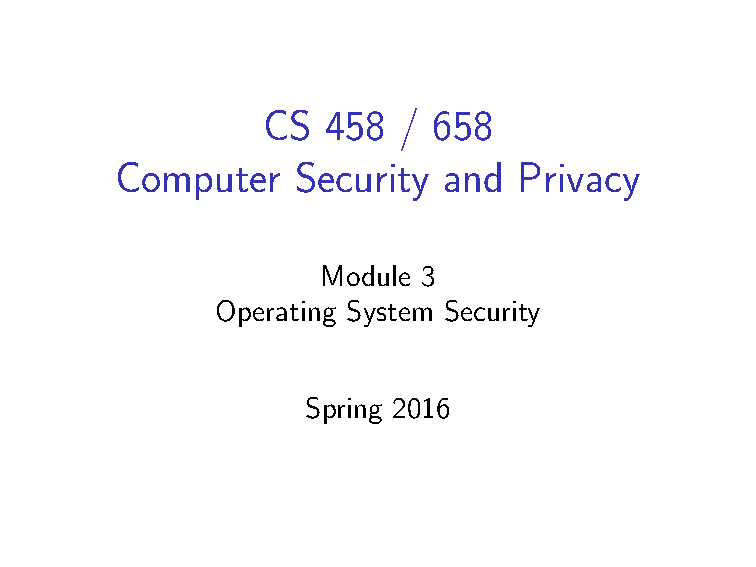
\includepdf[page=25]{Module3.pdf}
Capabilities are when we assign rights on a user basis (a row wise look at access matrix). Security for this is very hard because we have to have a list of rights stored somewhere. You have to maintain that when a user access it they don't fuck it up and have permission to look at it. This list can be stored on the OS or on the user, we prefer storing it on the OS. If we give a digital signature to a user (letting them store their own rights) you have to ask them for their capabilities whenever they want access. If a user is not contactable then we cannot know anything about them. It also makes it very hard to revoke their access because they can just refuse to give over their token.
 
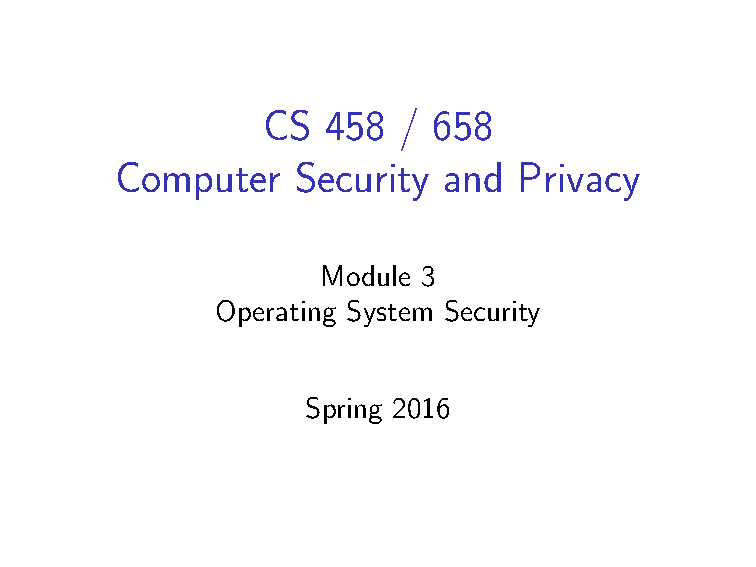
\includepdf[page=26]{Module3.pdf}
Most systems use a combination of the two primarily for performance reasons. In linux rights are originally stored as acls but when you open a file they get converted into capabilities (for example fopen returns a file descriptor that tells you its rights).

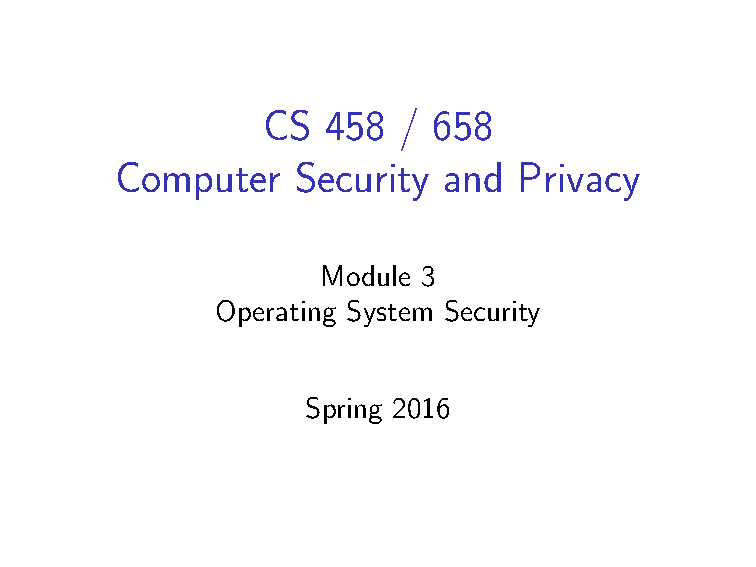
\includepdf[page=27]{Module3.pdf}
We like to clump users into groups called roles. Everyone in a role has the same access. This makes it very easy to update someones rights by just moving them to a new group. Most comercial databases use this model.

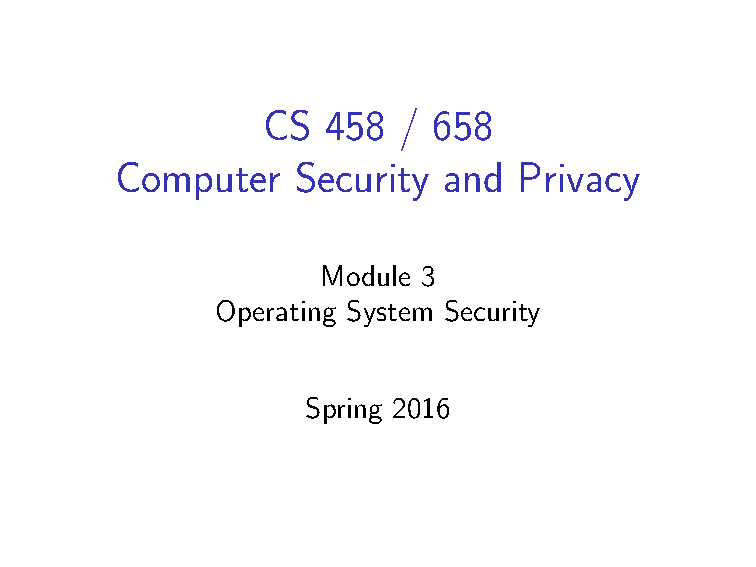
\includepdf[page=28]{Module3.pdf}

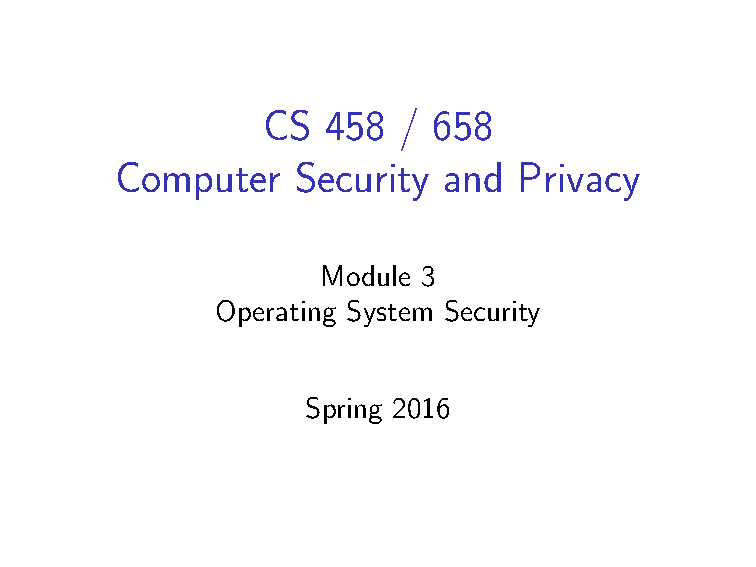
\includepdf[page=30]{Module3.pdf}
AUTHENTICATE EVERYTHING, yep thats pretty much it.

\textbf{Identification} is asking who someone is. \textbf{Authentication} is checking that you actually are who you say you are (make sure you have the rights you claim).

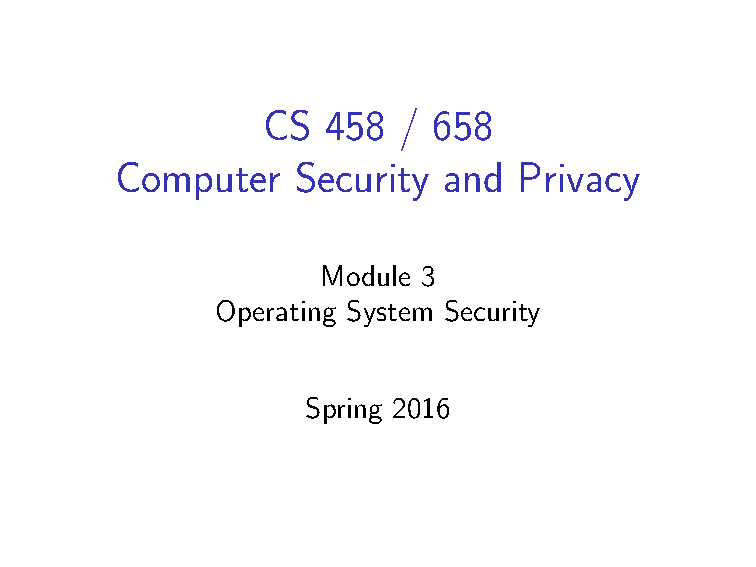
\includepdf[page=32]{Module3.pdf}
We can use what a user knows (some data they would know), what they have (an object they have like cookie or atm card), something about what the user is (like biometrics), and something about the user's context (like are they at home now).

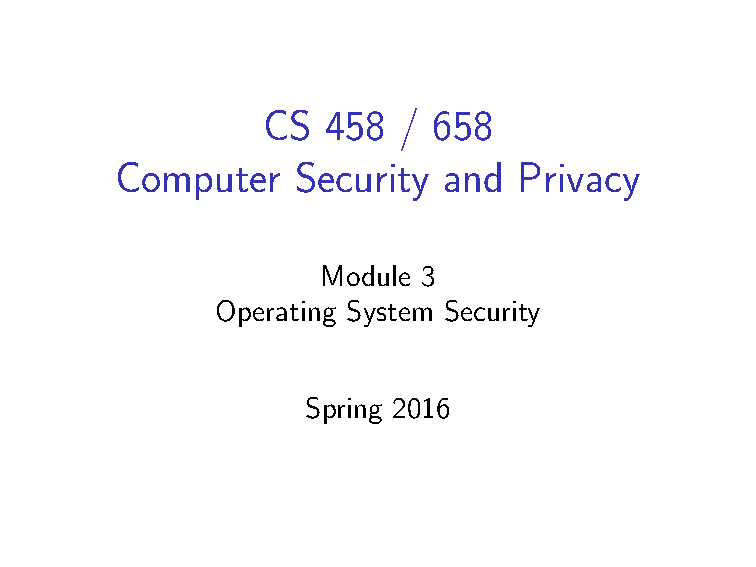
\includepdf[page=33]{Module3.pdf}
Good security usually looks to have multiple factors of authentication usually from different classes. With physical items we need to watch for them just becoming data. 







\end{document}